\chapter{Исследовательская часть}

\section{Технические характеристики}

Технические характеристики устройства, на котором выполнялся замерный эксперимент:
\begin{itemize}
	\item операционная система Ubuntu 22.04.1 LTS Linux x86\_64 \cite{ubuntu};
	\item память 8 ГБ;
	\item процессор Intel® Core™ i3-7130U.
\end{itemize}

Замеры проводилось на ноутбуке, включенном в сеть электропитания. Во время тестирования ноутбук был нагружен только встроенными приложениями окружения, окружением, а также непосредственно замерным экспериментом.

\section{Пример работы программы}

На рисунке \ref{img:example} представлен пример работы программы. Вводится количество вершин в графе и матрица смежности. Далее выводится матрица кратчайших путей и время выполнения последовательного и параллельного алгоритма в микросекундах. 

\begin{figure}[H]
	\centering
	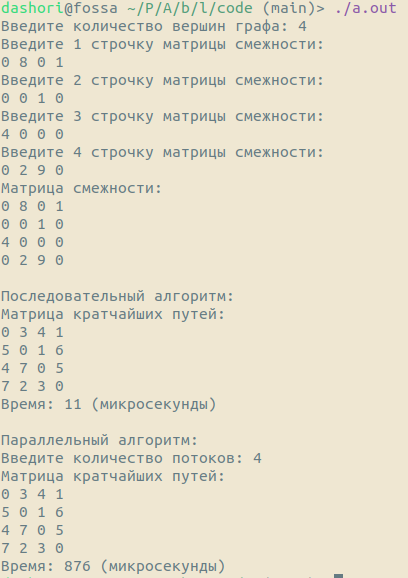
\includegraphics[width=120mm]{images/example}
	\caption{Пример работы программы}
	\label{img:example}
\end{figure}

Также при компиляции программы можно указать вывод графа на экран, но для графов с количеством вершин более 10 такой граф не является наглядным.
\begin{figure}[H]
	\centering
	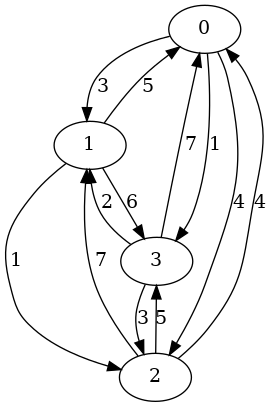
\includegraphics[width=60mm]{images/exampleGraph.png}
	\caption{Пример графа из тестовой программы}
	\label{img:example}
\end{figure}

\section{Время выполнения реализованных алгоритмов}

Было проведено два эксперимента по замеру времени. Первый -- зависимость времени работы реализованных алгоритмов от количества потоков, при это количество вершин графа фиксированно и равно 150. Второй -- зависимость времени  от количества вершин графа, при этом для параллельной реализации алгоритма количество потоков фиксировано и равно 4.

Замеры времени работы реализованных алгоритмов для каждого эксперимента проводились 200 раз. 
В таблице \ref{tab:time} представлен результат зависимости времени работы реализованных алгоритмов от количества вершин в графе, количество потоков для параллельной реализации равно 4.
\clearpage
\begin{table}[H]
	\begin{center}
		\begin{flushleft}
			\caption{\label{tab:time}Результаты замеров времени реализованных алгоритмов в микросекундах}
		\end{flushleft}
		\begin{tabular}{|l|l|l|l|l|}
			\hline \specialcell{Количество вершин\\в графе} & \specialcell{Последовательный\\алгоритм} &
			\specialcell{Параллельный\\алгоритм}  \\\hline
			1   & 0      & 428   \\ \hline
			11  & 99     & 162   \\ \hline
			21  & 548    & 617   \\ \hline
			31  & 1467   & 963   \\ \hline
			41  & 3401   & 1805   \\ \hline
			50  & 5831   & 3273   \\ \hline
			100 & 42865  & 20937   \\ \hline
			150 & 138661 & 67138   \\ \hline
			200 & 331876 & 156506     \\ \hline
		\end{tabular}
	\end{center}
\end{table}


В таблице \ref{tab:timeParallel} представлен результат зависимости времени работы реализованных алгоритмов от количества потоков, количество вершин графа равно 150.
\clearpage
\begin{table}[H]
	\begin{center}
		\begin{flushleft}
			\caption{\label{tab:timeParallel}Результаты замеров времени реализованных алгоритмов в микросекундах}
		\end{flushleft}
		\begin{tabular}{|l|l|l|l|l|}
			\hline \specialcell{Количество потоков} & \specialcell{Последовательный\\алгоритм} &
			\specialcell{Параллельный\\алгоритм}  \\\hline
			1  & 137489  & 132363 \\ \hline
			2  & 274394  & 203034 \\ \hline
			3  & 411187  & 284118 \\ \hline
			4  & 546128  & 349896 \\ \hline
			5  & 681251  & 420196 \\ \hline
			6  & 815748  & 488302 \\ \hline
			7  & 950798  & 555731 \\ \hline
			8  & 1094473 &  625521 \\ \hline
			9  & 1230592 &  693366 \\ \hline
			10 & 1367051 & 760079 \\ \hline
			11 & 1502139 & 826971 \\ \hline
			12 & 1637389 & 893409 \\ \hline
			13 & 1772377 & 960084 \\ \hline
			14 & 1907026 & 1028013 \\ \hline
			15 & 2042003 & 1093619  \\ \hline
			16 & 2176615 & 1160360  \\ \hline
		\end{tabular}
	\end{center}
\end{table}

На рисунке \ref{img:result} представлена зависимость времени работы реализованных алгоритмов Флойда от количества вершин в графе. На рисунке \ref{img:resultParallel} представлена зависимость времени работы реализованных алгоритмов Флойда от количества потоков.

\begin{figure}[H]
	\centering
	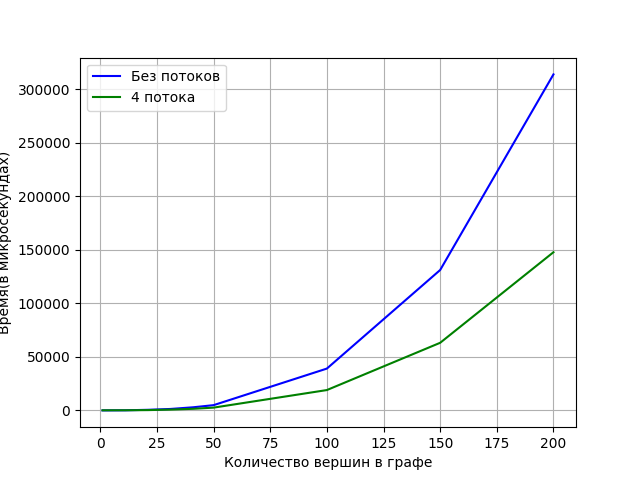
\includegraphics[width=140mm]{images/result}
	\caption{Зависимость времени работы реализованных алгоритмов Флойда от количества вершин в графе}
	\label{img:result}
\end{figure}
\begin{figure}[H]
	\centering
	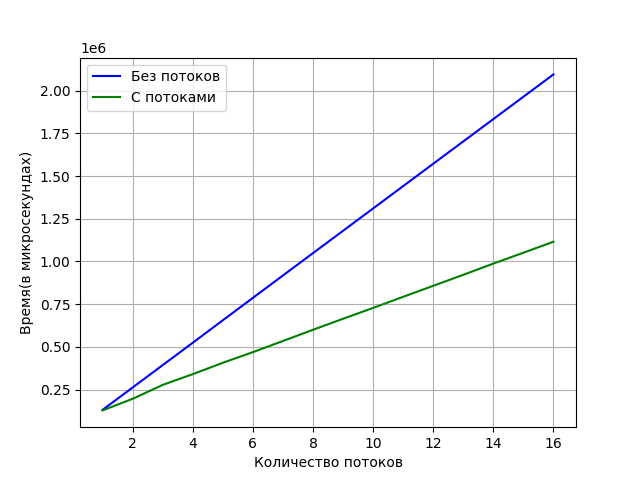
\includegraphics[width=140mm]{images/resultParallel}
	\caption{Зависимость времени работы реализованных алгоритмов сортировки от длины массива, где длина -- степень числа два}
	\label{img:resultParallel}
\end{figure}

\clearpage
Из рисунка \ref{img:result} видно особенность битонной сортировки, которая сортирует только массивы, длина которых является степенью числа два. Все массивы, имеющую иную длину, дополняются фиктивными элементами до ближайшей степени числа два, что видно на рисунке \ref{img:result}. 

Самая быстрая сортировка из исследуемых -- сортировка подсчетом. На размерах массива до 64 она превосходит в 8 раз битонную сортировку и в 3 раза сортировку слиянием. На размерах от 100 до 600 она работает быстрее в 30-50 чем битонная и в 6 раз быстрее чем сортировка слиянием. На максимальном тестируемом размере -- 65536 сортировка подсчетом быстрее битонной сортировки в 60 раз, а сортировки слиянием в 7 раз.  

Быстрая скорость сортировки подсчетом объясняется тем фактом, что она проигрывает по памяти двум другим алгоритмам сортировки, так как хранит дополнительный массив длина которого -- диапазон значений. Так как значения элементов массива генерировались произвольно в диапазоне\hspace{6mm}(-INT\_MAX,~INT\_MAX)~\cite{si}, исключается вариант, что сортировка подсчетом работает быстрее из-за тестовых данных. Также алгоритм битонной сортировки был реализован не параллельно, что ухудшает его трудоемкость.
